\chapter{Evaluation and Discussion}
\label{chap:eval}

\section{Available evidence}
This chapter reports the completed target-only baseline and defines the remaining comparisons. The archive contains 36 runs conducted on 13 October 2026, approximately 12:28--15:08 Moscow time~\cite{baseline}. All runs produced complete reports. Across the grid, 22,843 requests were submitted, 22,459 completed and 384 were cancelled; the separate error counter is zero. The overall cancellation fraction is 1.68\%, although cancellations are concentrated in particular conditions.

All numerical results below are derived from the archived JSON summaries and request-count CSV. Each condition has one measured run. There are no confidence intervals or optimized-model results in this draft. Full baseline percentiles and completion counts are provided in Appendix~\ref{app:baseline}.

\section{Performance at concurrency one}
Table~\ref{tab:c1} summarizes the closed-loop measurements. Median TTFT is between 12.71 and 13.89 ms, and median TPOT is between 6.50 and 6.59 ms. Median response latency increases with actual response length, while five of the six exported throughput measurements are close to 150--151 output tokens/s.

\begin{table}[htbp]
\centering
\caption{Baseline at concurrency one}
\label{tab:c1}
\begin{singlespace}
\small
\setlength{\tabcolsep}{4pt}
\renewcommand{\arraystretch}{1.2}
\begin{tabular}{@{}lrrrrr@{}}
\toprule
Profile & TPOT p50 & Latency p50 & Tokens/s & Output p50 & Done/sent \\
\midrule
RU 100 & 6.50 & 0.65 & 150.26 & 98 & 169/169 \\
EN 100 & 6.50 & 0.68 & 150.55 & 103 & 135/135 \\
RU 500 & 6.58 & 3.43 & 151.22 & 520 & 34/34 \\
EN 500 & 6.57 & 3.42 & 41.31 & 520 & 12/13 \\
RU 1000 & 6.59 & 5.82 & 151.14 & 882 & 22/22 \\
EN 1000 & 6.59 & 6.36 & 151.25 & 965 & 19/19 \\
\bottomrule
\end{tabular}
\par\smallskip\raggedright TPOT is in milliseconds; response latency is in seconds. Profile numbers denote requested output targets, not fixed lengths.
\end{singlespace}
\end{table}


The English 500-token condition is an exception: it reports 41.31 tokens/s, with 12 completed requests out of 13 submitted. Its median TPOT remains 6.57 ms. This result must not be interpreted as evidence of a slower decoding kernel. The small sample, cancellation and metric observation window require investigation using raw traces and a repeated run. The archived summaries alone do not establish the cause.

The requested output target also does not bound observed length. In the English 100-token, concurrency-one run, the median is 103 tokens but p99 is 1266.60 tokens. This long tail contributes to the difference between typical and tail response latency. In addition, the 500- and 1000-token concurrency-one runs contain only 12--34 completed requests each, limiting the interpretation of high percentiles.

\pending{E0: repeat the baseline, investigate the English 500-token anomaly and retain request traces. Add uncertainty estimates before using these measurements as final speedup denominators.}

\section{Behavior as offered load increases}
Figure~\ref{fig:throughput} shows the five open-loop load levels. Aggregate throughput increases across the tested rates for all six profiles. This increase reflects more work completed per unit time and should be considered together with individual-request latency and completion fraction.

\begin{figure}[htbp]
\centering
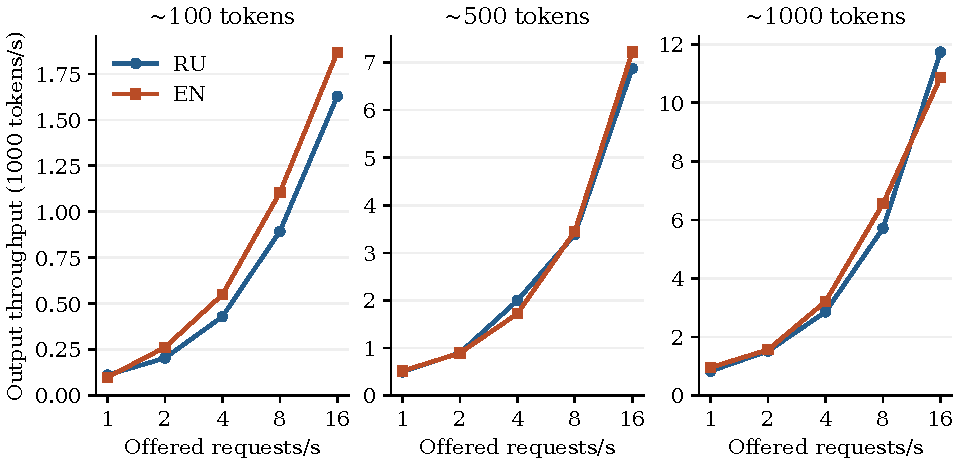
\includegraphics[width=\textwidth]{baseline_throughput.pdf}
\caption[Baseline throughput versus offered load]{Exported baseline output throughput versus offered RPS. Each point is one run; lines connect measured conditions. Output targets are instructions, not fixed lengths.}
\label{fig:throughput}
\end{figure}

At 16 RPS, the 100-token profiles complete all submitted requests and have p99 TTFT below 27 ms. The 500-token profiles reach 6876.25 tokens/s in Russian and 7219.03 tokens/s in English, with a small number of cancellations. The 1000-token profiles incur much greater response latency, as shown in Table~\ref{tab:load16}.

\begin{table}[htbp]
\centering
\caption{Baseline at 16 offered requests/s}
\label{tab:load16}
\begin{singlespace}
\small
\setlength{\tabcolsep}{4pt}
\renewcommand{\arraystretch}{1.2}
\begin{tabular}{@{}lrrrr@{}}
\toprule
Profile & TTFT p99 (ms) & Latency p99 (s) & Tokens/s & Done/sent \\
\midrule
RU 100 & 25.73 & 2.54 & 1628.00 & 1878/1878 \\
EN 100 & 26.50 & 3.78 & 1866.97 & 1955/1955 \\
RU 500 & 39.74 & 8.70 & 6876.25 & 1953/1956 \\
EN 500 & 41.94 & 10.98 & 7219.03 & 1950/1952 \\
RU 1000 & 99.37 & 26.33 & 11729.77 & 1936/1938 \\
EN 1000 & 12180.92 & 62.72 & 10856.48 & 1626/1972 \\
\bottomrule
\end{tabular}

\end{singlespace}
\end{table}


The English 1000-token profile is the clearest high-load concern. Between 8 and 16 RPS, median TPOT rises from 11.19 to 31.23 ms and p99 TTFT rises from 53.20 ms to 12.18 s. At 16 RPS, 346 of 1972 submitted requests are cancelled: only 82.45\% complete. The p99 response latency of completed requests is 62.72 s. Figure~\ref{fig:tail} presents this change alongside completion fraction.

\begin{figure}[htbp]
\centering
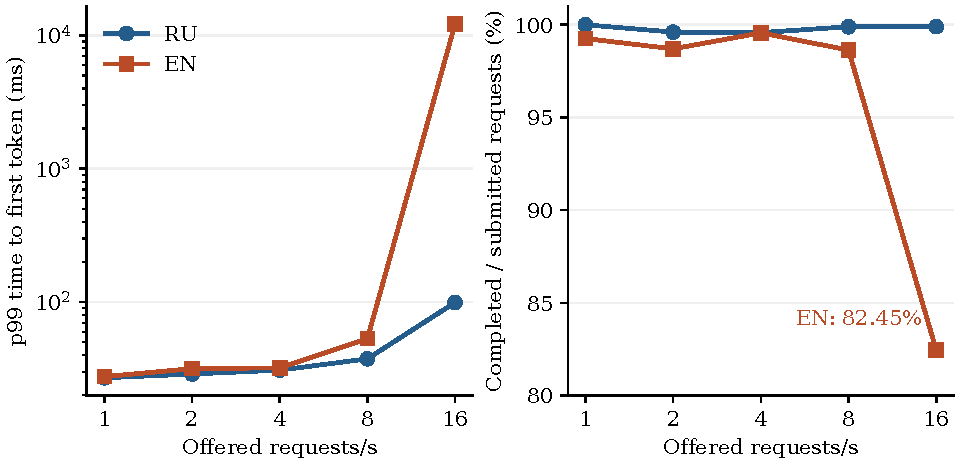
\includegraphics[width=\textwidth]{baseline_tail.pdf}
\caption[Tail latency and completion for long responses]{The 1000-token profiles: p99 TTFT for completed requests and completion fraction. The TTFT axis is logarithmic. Cancelled requests are absent from latency percentiles.}
\label{fig:tail}
\end{figure}

These observations are consistent with substantial serving pressure in that condition, but they do not isolate its cause. Queue traces and GPU profiling are needed to distinguish scheduling, memory, compute and host-side effects. The Russian 1000-token condition reaches 11,729.77 tokens/s at 16 RPS with 1936 of 1938 requests completed, but its p99 response latency is still 26.33 s. Different generated lengths and prompt contents prevent treating this comparison as a controlled language effect.

The tested grid does not establish a maximum sustainable request rate. That claim would require longer runs, predefined latency and completion targets, and finer sampling around the capacity boundary. High throughput alone is insufficient when a sizeable share of work remains unfinished.
\FloatBarrier

\section{Planned optimization comparisons}
The central thesis results will extend the baseline in this chapter. Each retained configuration will receive the complete 36-condition table, including acceptance metrics where applicable. Comparisons will report both typical and tail latency, throughput, output lengths and completion counts. Peak GPU memory and quality scores will be added when measured.

\begin{table}[htbp]
\centering
\caption{Experiments required to complete the evaluation}
\label{tab:pending}
\begin{singlespace}
\small
\begin{tabularx}{\textwidth}{@{}p{1.1cm}p{3.6cm}X@{}}
\toprule
ID & Comparison & Result to insert \\
\midrule
E1 & Tuned engine vs. $B_0$ & Configuration search, retained $B_1$, latency and throughput changes. \\
E2 & DFlash vs. matched control & Draft-cost and acceptance analysis, workload-specific gains or regressions. \\
E3 & Quantization vs. BF16 & Precision, calibration, quality change, memory and performance. \\
E4 & Profile-guided changes & Bottleneck evidence, selected kernel or scheduler change, end-to-end effect. \\
E5 & Combined pipeline & Full configuration and component-removal results against $B_0$ and $B_1$. \\
E6 & Workload-based selection & Held-out evaluation of configuration rules and their failure cases. \\
\bottomrule
\end{tabularx}
\end{singlespace}
\end{table}

\pending{E1--E4: insert per-method tables and explain both improvements and regressions. Report measured speedups without assuming that published gains transfer to this setup.}

\pending{E5: insert the cumulative comparison and component-removal figure. Quantify whether combined gains are additive, smaller than expected or workload dependent.}

\pending{E6 and Q1: insert held-out workload and quality results. State the final selection rule only after its validation.}

\section{Current answers to the research questions}
For RQ1, the baseline provides reference measurements; achievable acceleration remains pending until the combined pipeline and matched controls are evaluated. For RQ2, interactions between speculation, precision and execution require individual and component-removal experiments. For RQ3, load and response profile clearly affect baseline behavior, but a configuration-selection rule has not yet been validated.

The baseline shows why throughput, tail latency and completion must be reported together. It establishes no optimized speedup, quality-preservation result or memory reduction. Those claims will depend on the remaining experiments and their uncertainty estimates.
